%!TEX root = ../Electrodynamics.tex
\subsection{Затухание волн в линии передач, обусловленное потерями энергии в металлической стенке.}
\begin{figure}[h!]
	\centering
	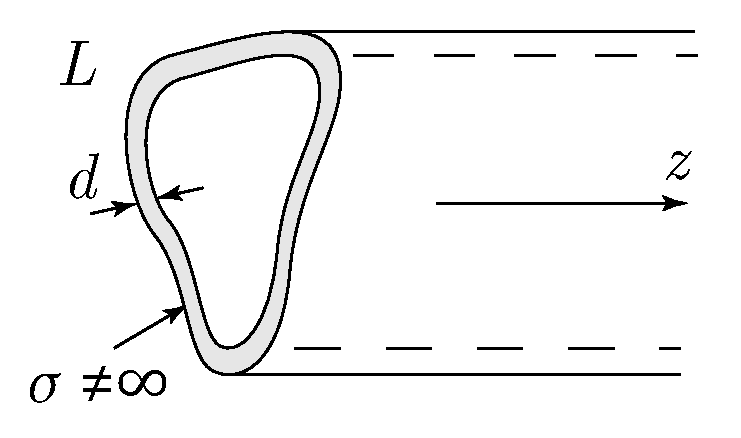
\includegraphics[width = 0.4\linewidth]{img/9-1-1.pdf}
	\caption{ЛП с неидеальными стенками}
\end{figure}
Имеется полая ЛП, заполненная либо $\epsilon,\mu$, либо ничем. Стенки сделаны из хорошего, но не идеального проводника:
\begin{align*}
	&\epsilon_{wall} = \epsilon' +i\epsilon''\\
	&w\ll 4\pi \sigma, \epsilon'' = -\frac{4\pi\sigma}{w} \Rightarrow |\epsilon_{wall}''|>|\epsilon_{wall}'|\\
	&\epsilon \approx -i \frac{4\pi \sigma}{w}, |\epsilon''|\gg 1
\end{align*}
На поверхности хорошего проводника выполняется граничное условие Леонтовича.
\begin{equation}
	\vec{E}_{\tau} = \eta_s\left[\vec{H}_{\tau} \times \vec{n}\right]	,
\end{equation}
$\eta_s$ - поверхностный импеданс.
В проводнике волна быстро затухает:
\begin{equation}
	E_x \sim e^{-\frac{1+i}{\delta}x}e^{iwt},~ \delta = \frac{c}{\sqrt{8\pi\sigma\mu w}},
\end{equation}
где $\delta$ - толщина скин-слоя, $k = \frac{1+i}{\delta}$ - волновое число в стенке. 
Поля слева от границы удовлетворяют граничному условию:
\begin{equation}
	\vec{E}_{\tau} = \eta_s\left[\vec{H}_{\tau} \times \vec{n}\right]	,
\end{equation}
$\vec{n}$ - нормаль вглубь проводника. При этом:
\begin{equation}
	\eta_s = \sqrt{\frac{\mu_{wall}}{\epsilon_{wall}}} = \sqrt{i\frac{w\mu_{wall}}{4\pi\sigma}}
\end{equation}
Это точное решение в случае, когда рассматривается бесконечная металлическая полуплоскость. У нас толщина проводника
конечная, и для использования г.у. Леонтовича нужны дополнительные ограничения на параметры стенки $d$.

Во-первых, толщина стенки должна быть много больше толщины скин-слоя, чтобы волны успели затухнуть. Во-вторых, так как
мы  изначально не накладывали ограничений на форму стенки, она может быть произвольной формы, а значит и структура поля внутри
проводника будет различной для разных участков поверхности. Чтобы рассматривать малые участки как линейные, необходимо,
чтобы радиус кривизны поверхности был много больше толщины скин-слоя. В итоге получаем 3 условия:
\begin{equation}
	\sigma\gg w, ~ \delta \ll R_{\text{кр}}, ~ \delta \ll d
\end{equation}
В таком случае можно пользоваться г.у. Леонтовича.

Рассмотрим участок ЛП от $z$ до $z+\Delta z$. При распространении, часть энергии волны диссипатирует в стенках:
\begin{align*}
	& \Pi(z) = \Pi(z+\Delta z)+\Delta P_{wall}\\
	& \Delta P_{wall} = P_{wall}\Delta z,
\end{align*}
где $ P_{wall}$ - количество энергии, потерянное в стенках на единицу длины (погонная мощност потерь), а $\Pi$ - мощность волны.
\begin{equation}
	P_{wall} = -\frac{\Pi(z+\Delta z)-\Pi(z)}{\Delta z},~\Delta z \to 0,	
\end{equation}
\begin{equation}
	P_{wall} = -\frac{\dd \Pi}{\dd z} - \text{дифференциальный ЗСЭ}
\end{equation}
Рассмотрим поля в ЛП:
\begin{align*}
	&\vec{E},\vec{H} \sim e^{-ihz},~ h =h'+ih''\\
	&|\vec{E}|,|\vec{H}| \sim e^{h''z}
\end{align*}
Здесь везде речь идет о среднем потоке энергии!
\begin{align*}
	&\Pi \sim |\vec{E}|,|\vec{H}|\sim e^{2h''z} \Rightarrow\\
	& \Rightarrow \frac{\dd \Pi}{\dd z} = 2h'' \Pi \Rightarrow h'' = -\frac{P_{wall}}{2 \Pi}
\end{align*}
\begin{figure}[h!]
	\centering
	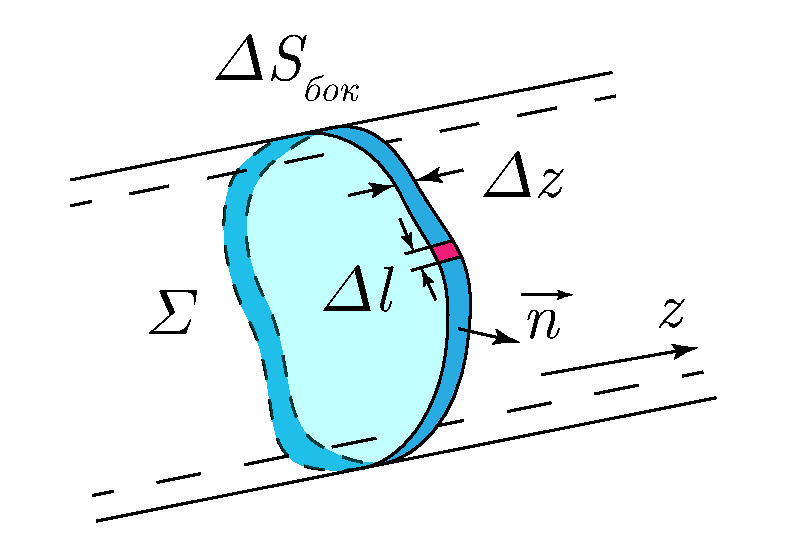
\includegraphics[width = 0.4\linewidth]{img/9-1-3.pdf}
	\caption{иллюстрация к интегралу по площади}
\end{figure}
При переходе здесь пользуясь граничным условием Леонтовича получим:
\begin{align*}
	\Delta P_{wall} = \iint \limits_{S_{\text{бок}}} &\bar{S}_n \dd S = \iint \limits_{S_{\text{бок}}} \frac{c}{8\pi} \Re{\left[\vec{E}\times\vec{H}^*\right]}_n\dd S =\\
	&  = \frac{c}{8\pi}\oint \limits_L \Re{\eta_s} |\vec{H}_{\tau}|^2 \dd l \Delta z,
\end{align*}
и тогда выражение для $h''$ принимает вид:
\begin{equation}
	h'' = -\frac{P_{wall}}{2 \Pi} = -\frac{\Re{\eta_s} \oint \limits_L  |\vec{H}_{\tau}|^2 \dd l}{2 \Re{\eta_{\perp_{\text{в}}}} \iint \limits_{\Sigma}|\vec{H}_{\perp}|^2 \dd S}	
\end{equation}
Можно ввести $L_{\text{затух}}$ - расстояние, на котором амплитуда колебнаия спадает в $e$ раз:
\begin{equation}
	|h''| = \frac{1}{L_{\text{затух}}}	
\end{equation}
%%%%%%%%%%%%%%%%%%%%%%%%%%%%%%%%%%%%%%%%%%%%%%%%%%%%%%%%%%%%%%%%%%%%%%%%%%%%%%%%%%%%%%%%%%%%%%%


\subsection{Лемма Лоренца и теорема взаимности для двух систем монохроматических источников.}
\textbf{Лемма Лоренца}

Эта лемма относится к гармоническим полям и токам
\begin{equation}
	\vec{E},\vec{H},\vec{j}\sim e^{iwt}
\end{equation}
Рассмотрим две системы источников (токи, в общем случае, и магнитные $\vec{j}^m$) в одинаковой среде $\epsilon,\mu$.
Токи пораждают соответствующе поля:
\begin{align*}
	&\vec{j}^{e,m}_1 \sim e^{iwt} \rightarrow \vec{E}_1,\vec{H}_1,\vec{j}\sim e^{iwt}\\
	&\vec{j}^{e,m}_2 \sim e^{iwt} \rightarrow \vec{E}_2,\vec{H}_2,\vec{j}\sim e^{iwt}
\end{align*}
Частота $w$ этих источников одинаковая - эти источники \textbf{монохроматические}. Мы можем записать уравнения Максвелла
в общем виде, с учетом фихтивных токов:
\begin{align*}
	&\Rot{\vec{H}_1} = \frac{4\pi}{c}\vec{j}^{e}_1 + \frac{iw}{c}\epsilon\vec{E}_1|\cdot\vec{E}_2\\
	&\Rot{\vec{E}_1} = -\frac{4\pi}{c}\vec{j}^{m}_1 - \frac{iw}{c}\epsilon\vec{H}_1|\cdot\vec{H}_2\\
	&\Rot{\vec{H}_2} = \frac{4\pi}{c}\vec{j}^{e}_2 + \frac{iw}{c}\epsilon\vec{E}_2|\cdot\vec{E}_1\\
	&\Rot{\vec{E}_2} = -\frac{4\pi}{c}\vec{j}^{m}_2 - \frac{iw}{c}\epsilon\vec{H}_2|\cdot\vec{H}_1
\end{align*}
Используя соотношение:
\begin{equation}
	\Div{\left[\vec{A} \times \vec{B} \right]} = \vec{B}\Rot{\vec{A}} - \vec{A}\Rot{\vec{B}}
\end{equation}
преобразуем 4 уравнения выше, складывая все уравнения. В итоге получим:
\begin{align*}
	\Div{\left[\vec{E}_1 \times \vec{H}_2\right]} - &\Div{\left[\vec{E}_2 \times \vec{H}_1\right]} = \\
	& = \frac{4\pi}{c}\left( \vec{j}^{e}_1 \vec{E}_2-\vec{j}^{m}_1 \vec{H}_2-\vec{j}^{e}_2 \vec{E}_1+\vec{j}^{m}_2 \vec{H}_1 \right)
\end{align*}
Далее, интегрируем по произвольному объему, охватывающему эти источники, и применяя формулу Гаусса-Остроградского
получим:
\begin{align*}
	\oiint \limits_S \left[\vec{E}_1 \times \vec{H}_2 \right] - &\left[ \vec{E}_2 \times \vec{H}_1\right] \vec{n} \dd S =\\
	&=\frac{4 \pi}{c} \int \limits_V \left( \vec{j}^{e}_1 \vec{E}_2-\vec{j}^{m}_1 \vec{H}_2-\vec{j}^{e}_2 \vec{E}_1+\vec{j}^{m}_2 \vec{H}_1 \right) \dd V
\end{align*}
Это соотношение и есть формулировка \textbf{леммы Лоренца}. Такие соотношения позволяют связывать решения двух разных
задач, зная решение простой задачи, можно решить сложную.

\begin{figure}[h!]
	\centering
	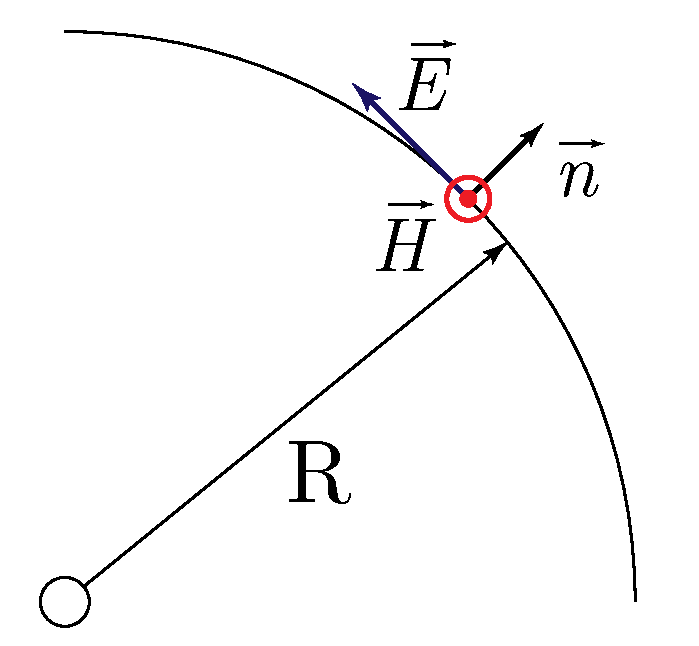
\includegraphics[width = .4\linewidth]{9-2.pdf}
	\caption{К теореме взаимности}
\end{figure}
\textbf{Теорема взаимности}

Распространим объем $V\to\infty$ в лемме Лоренца. В таком случае поверхностью интегрирования $S$ может быть сфера
радиуса $R\to\infty$.

Источники обеих систем ограничены в пространстве. При большом удалении, поля от источников представляют собой
сферические волны. У сферической волны, на бесконечности можно рассматривать ее малый участок как плоский, тогда волны
будут чисто поперечными. Волновое сопротивление среды:
\begin{equation}
	\frac{E_{\perp}}{H_{\perp}} = \eta_{\text{в}} = \sqrt{\frac{\mu}{\epsilon}}	
\end{equation} 
Выражение выше - приближение характер, однако при устремлении $R\to\infty$, его точность увеличивается. Тогда имеем:
\begin{equation}
	\vec{E}_{1,2} = \eta_{\text{в}} \left[\vec{H}_{1,2} \times \vec{n}\right]	,
\end{equation}
где $\vec{n}$ - направление распространения волны (внешняя нормаль к $S$). $\eta_{\text{в}}$ - одинакова для систем
источников 1 и 2. Тогда справедливо:
\begin{align*}
	\left[\vec{E}_{1} \times \vec{H}_2 \right] = \eta_{\text{в}} \left[ \left[\vec{H}_{1} \times \vec{n}\right]\times \vec{H}_2\right] = \eta_{\text{в}} \left(\vec{n}(\vec{H}_1,\vec{H}_2) - \vec{H}_2\underbrace{(\vec{H}_1,\vec{n})}_{=0}\right) 
\end{align*}
\begin{equation}
	\left.
	\begin{aligned}
		&\left[\vec{E}_{1} \times \vec{H}_2 \right] = \eta_{\text{в}} \vec{n} (\vec{H}_1,\vec{H}_2)\\
		&\left[\vec{E}_{2} \times \vec{H}_1 \right] = \eta_{\text{в}} \vec{n} (\vec{H}_2,\vec{H}_1)
	\end{aligned}
	\right\} \left[\vec{E}_{1} \times \vec{H}_2 \right] - \left[\vec{E}_{2} \times \vec{H}_1 \right] \equiv 0
\end{equation}

Т.е. левая часть в лемме Лоренца \underline{при большом расстоянии} равна нулю. Это верно с точночтью до членов порядка
$\frac{1}{R^2}$. Оставшийся в правой части интеграл разделим на два, таким образом, получаем
формулировку \textbf{тоеремы взаимности}:
\begin{align*}
	&\int \limits_V \left( \vec{j}^{e}_1 \vec{E}_2-\vec{j}^{m}_1 \vec{H}_2-\vec{j}^{e}_2 \vec{E}_1+\vec{j}^{m}_2 \vec{H}_1 \right) \dd V = 0\\
	&\int \limits_V \left( (\vec{j}^{e}_1,\vec{E}_2)-(\vec{j}^{m}_1,\vec{H}_2)\right) \dd V = \int \limits_V\left( (\vec{j}^{e}_2,\vec{E}_1)-(\vec{j}^{m}_2,\vec{H}_1) \right) \dd V
\end{align*}
Эта теорема также используется для сведения сложных задач к простым. \textbf{Условия выполнения теоремы}:
\begin{itemize}
	\item Среды должны быть линейными, $\epsilon,\mu$ - не должны зависить от полей.
	\item Рассматриваем изотропную среду
\end{itemize}
